

\documentclass[a4paper,10pt]{book}
%\documentclass[a4paper,10pt]{scrartcl}

\usepackage[utf8x]{inputenc}
\usepackage{fullpage}
\usepackage[final]{pdfpages}
\usepackage{wrapfig}
\usepackage{amssymb}
\usepackage{amsmath}
\usepackage{amsfonts}
\usepackage{amsbsy}
\usepackage{hyperref}
\usepackage{cite}
\graphicspath{{./documentation_images/}}
\usepackage{subfigure}
\usepackage{graphicx}
\usepackage[rightcaption]{sidecap}
%\usepackage{breqn}
%\usepackage{dsfont}
\usepackage{listings} %for writing code in the document
\setlength{\parindent}{0cm}
\usepackage{todonotes}
\usepackage{color,soul}
\usepackage{bm}

% TODO notes
\newcommand{\hlcom}[2]{\hl{#1} \todo{#2}}

%for blank pages
\usepackage{afterpage}

\newcommand\blankpage{%
	\null
	\thispagestyle{empty}%
	\addtocounter{page}{-1}%
	\newpage}




\title{Documentation for DISCO: the swain lab segmentation software}
\author{Elco Bakker}

\begin{document}
\maketitle
\section{Introduction}
\label{sec:intro}
 
 Welcome to the DISCO software: a software for segmenting yeast cells in trap like microfluidic devices, tracking them and viewing/editing the results. First, a few notes:
 \begin{itemize}
 	\item The software requires that the swain lab general functions package also be installed, which can be found at \href{https://github.com/pswain/GeneralMatlabFunctions}{https://github.com/pswain/GeneralMatlabFunctions}. \\
 	If you installed/pulled the software from the link \href{https://github.com/pswain/DISCO}{https://github.com/pswain/DISCO}, this should already be included as a folder called \texttt{GeneralMatlabFunctions}.
 	\item The best description of the underlying algorithm is the associated paper published at\\ \href{https://academic.oup.com/bioinformatics/article-abstract/doi/10.1093/bioinformatics/btx550/4103414?redirectedFrom=fulltext}{https://academic.oup.com/bioinformatics/article-abstract/doi/10.1093/bioinformatics/btx550/4103414?redirectedFrom=fulltext}.
 	\item The software was developed in the swain lab, and you should feel free to contact them with help and support in using the software (\href{http://swainlab.bio.ed.ac.uk/}{http://swainlab.bio.ed.ac.uk/}).
 	\item It is recommended that you use the software with MATLAB 2015b. Using it with later versions of matlab requires some extra setup steps that are detailed in section \ref{sec:other_matlabs}.
 \end{itemize}
 
 There are broadly two parts to the software: using the software to segment images and training the software to segment unseen image types. The first, segmenting, is relatively straightforward and is how you will use the software day to day. The second, training, requires a little more expertise and effort but should only need to be done once for a given imaging modality/microscope. \\
 We will first describe segmentation, and then describe training, even though it may be necessary for somebody in your group to train a model before anyone is able to segment images.
\section{Segmenting Timeseries Using the DISCO software}
\label{sec:segmenting_timeseries}
DISCO is a comprehensive (we hope) software for automatically segmenting cells in trap like devices and inspecting/editing the result. The processing is done through a combination of a matlab script, which is run cell by cell, and a collection of GUI's. We have found that this combination allows people to customise their personal work flows and allows the software to be easily updated and maintained. The standard work flow is:
\begin{enumerate}
	\item The user points the software to the images that make up the experiment and provides some basic information about the experiment.
	\item The user checks the identification of traps in the images and sets a number of parameters, mostly by GUI.
	\item The software uses a \textbf{cellVision Model} and \textbf{cellMorphology Model} to automatically identify and track cells in the images.
	\item The user can at this stage check and edit the automated cell identification and tracking and select cells to exclude from the data extraction.
	\item The software extracts data for the selected cells which can be used in analysis.
\end{enumerate}

\section{Using DISCO with Other Systems}

\subsection{Getting DISCO to read your files}
\begin{figure}
	\centering
	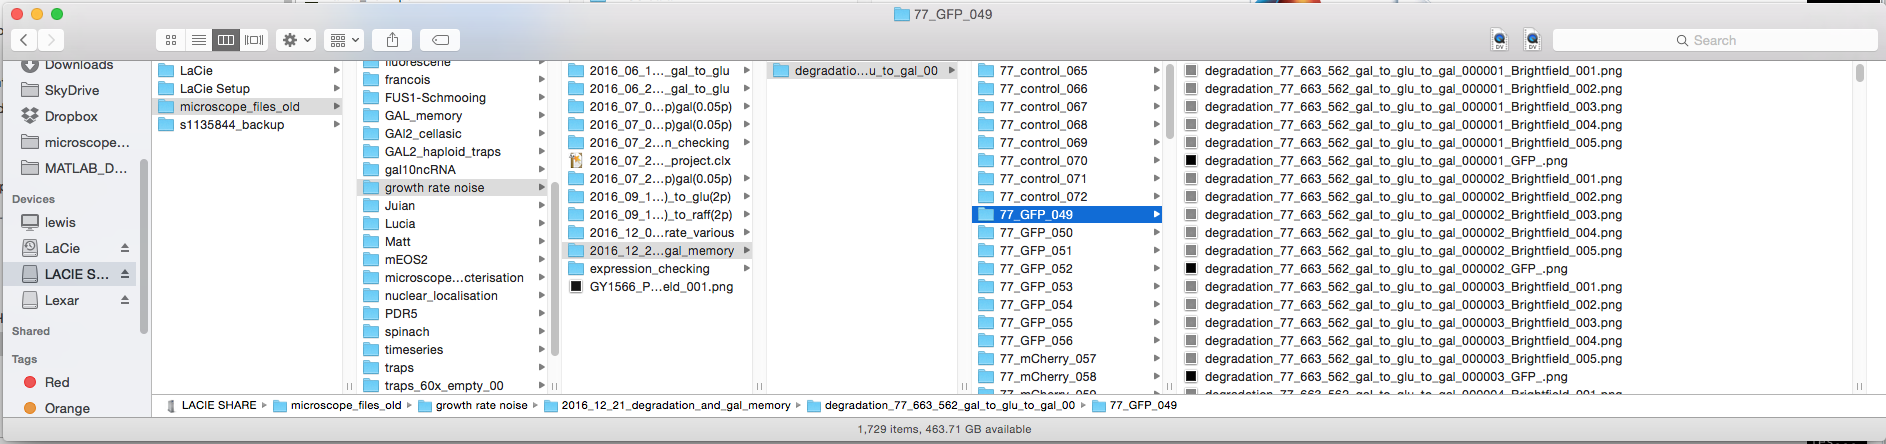
\includegraphics[width=1\linewidth]{documentation_images/other_systems-swain_file_structure}
	\caption[swain lab image file system]{An example of how images are stored in the swain lab image file system. The example shows and experiment called \texttt{degradation\_77\_663\_562\_gal\_to\_glu\_to\_gal\_00} in which Brightfield was imaged with 5 z slices and GFP was imaged with only 1. }
	\label{fig:other_systems-swain_file_structure}
\end{figure}
In order to be able to process the images in anyway, DISCO must of course be able to load your files and therefore know where they are.\\
The DISCO software was designed to be used with files generated by the swain lab microscope control software, which stores files in the form:
\begin{verbatim}
[experiment name]_[6 character timepoint]_[channel name]_[3 character z-slice].png
\end{verbatim}
with each position being stored in a separate folder. An example is shown in figure \ref{fig:other_systems-swain_file_structure}. This is (I believe) also the convention followed by MicroManager. If you're files are arranged in a different structure an you wish to make the software work, there are two options open to you.

\subsubsection{Easy Option: Export Images using ImageJ}
\begin{figure}
\centering
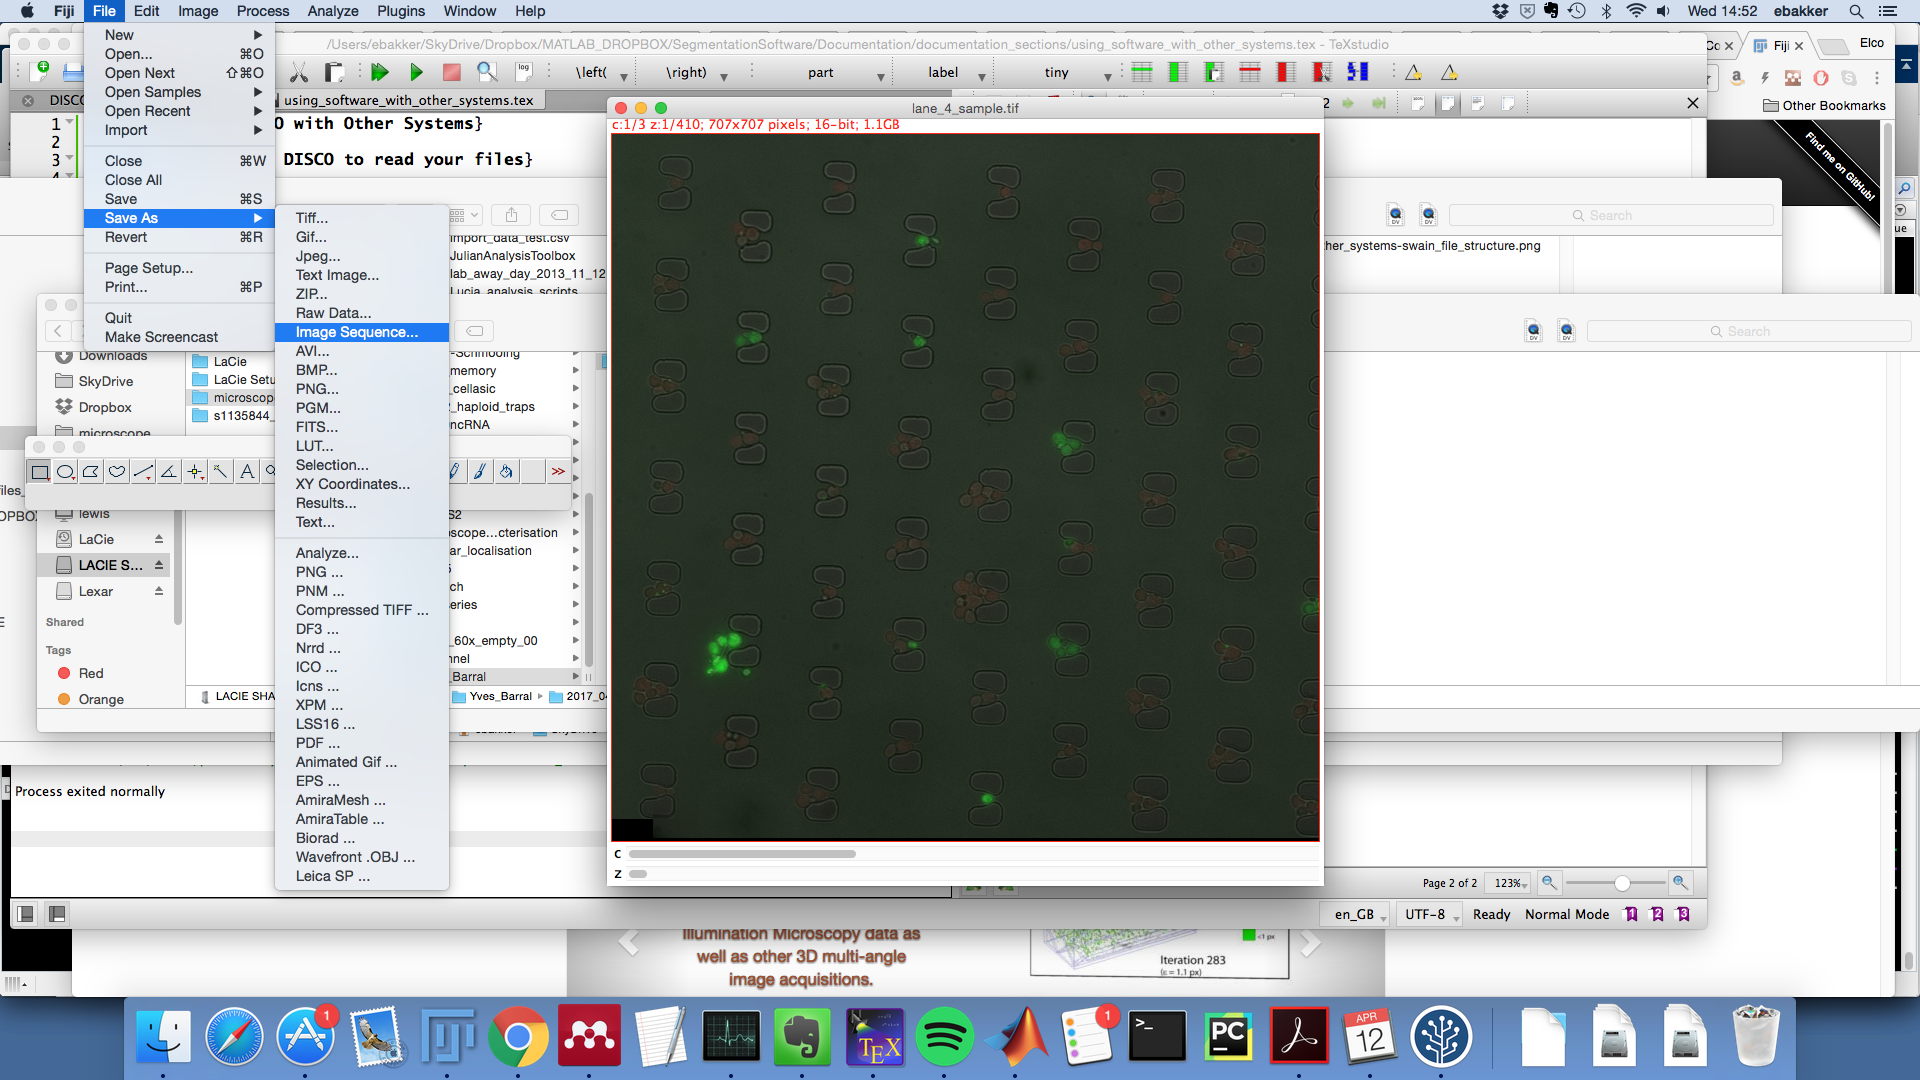
\includegraphics[width=1\linewidth]{documentation_images/other_systems-exporting_from_FIJI}
\caption[Exporting images for processing from FIJI]{Exporting images for processing from FIJI. Shown is the `save' options that should be selected for exporting an image stack for processing from FIJI. Selecting this option will open a dialogue box in which `format' should be set to PNG and `digits' should be set to 6.}
\label{fig:other_systems-exporting_from_FIJI}
\end{figure}


The easiest option is to use ImageJ or \href{https://fiji.sc/}{FIJI} to save your images in this format. These programs can handle most image formats and file structures.\\
First load in an images stack in a way you are happy with. Then save the image stack as an image sequence, choosing a format of PNG and Digits as 6. This will store the image sequence in format appropriate for the software, with channel names given as \texttt{c000001,c000002,c000003 ...}\\
If multiple image stacks are to be processed they can be saved to separate folders in the same parent folder (in imitation of the Swain Lab file structure), allowing the software to be conveniently run on all of them.

\subsubsection{Developer Option: Modify \texttt{timelapseTraps} Constructor and \texttt{timelapseTraps.addChannelsTimelapse} method.}



 \bibliographystyle{apalike}
 \bibliography{./library.bib}

%
\end{document}


